\documentclass{beamer}

\def\Tiny{\fontsize{6pt}{6pt}\selectfont}
\def\supertiny{\fontsize{4pt}{4pt}\selectfont}

\mode<presentation>
{
  \usetheme{Warsaw}
  % \setbeamercovered{transparent}
  \usecolortheme{crane}
}

\usepackage{graphicx, ifthen, listings, fancyvrb}

\usepackage[czech]{babel}
% \usefonttheme{professionalfonts}
\usepackage{times}
\usepackage{amsmath}
\usepackage[utf8]{inputenc}
\usepackage{wrapfig}

\usepackage[T1]{fontenc}

\lstset{ basicstyle=\tiny, stringstyle=\ttfamily, showstringspaces=false }

\everymath{\displaystyle}

\setbeamerfont{frametitle}{size=\large}
\setbeamerfont{subsection in toc}{size=\scriptsize}

\makeatletter\newenvironment{blackbox}{%
   \begin{lrbox}{\@tempboxa}\begin{minipage}{0.95\columnwidth}}{\end{minipage}\end{lrbox}%
   \colorbox{black}{\usebox{\@tempboxa}}
}\makeatother

\title[IMF (9)]{Informatika pro moderní fyziky (9)\\ inteligentní šablony, procvičení ERb+LaTeX, tvorba vektorové grafiky}

\author[Franti\v{s}ek HAVL\r{U}J, ORF ÚJV Řež]{Franti\v{s}ek HAVL\r{U}J\\{\scriptsize \emph{e-mail: haf@ujv.cz}}}

\date{akademický rok 2017/2018\\6. prosince 2017}

\institute[ORF ÚJV Řež]
{ÚJV Řež\\oddělení Reaktorové fyziky a podpory palivového cyklu}

\AtBeginSection[]
{
\begin{frame}<beamer>
\frametitle{Obsah}
\tableofcontents[currentsection,hideothersubsections]
\end{frame}
}

\begin{document}

\begin{frame}
  \titlepage
\end{frame}

\begin{frame}
  \tableofcontents
\end{frame}

\section{Na šablony chytře}

\begin{frame}{Úskalí šablon}
  \begin{itemize}
    \item snadno umíme nahradit jeden řetězec druhým
    \item trochu méně pohodlné pro větší bloky textu
    \item navíc by se hodila nějaká logika (cyklus) přímo v~šabloně
    \item naštěstí jsou na to postupy
  \end{itemize}
\end{frame}

\begin{frame}{ERb (Embedded Ruby)}
  \begin{itemize}
    \item lepší šablona - ``aktivní text''
    \item používá se například ve webových aplikacích
    \item hodí se ale i na generování latexových dokumentů, resp. všude, kde nám nesejde na whitespace
    \item poměrně jednoduchá syntax, zvládne skoro všechno (viz předmět MAA3)
  \end{itemize}
\end{frame}


\begin{frame}[fragile]{Základní syntaxe ERb (1)}
  \begin{block}{ }
    Jakýkoli Ruby příkaz, přiřazení, výpočet ...
    \scriptsize
    \begin{verbatim}
      <% a = b + 5 %>
      <% list = ary * ", " %>
    \end{verbatim}
  \end{block}
\end{frame}

\begin{frame}[fragile]{Základní syntaxe ERb (2)}
  \begin{block}{ }
    Pokud chci něco vložit, stačí přidat rovnítko
    \scriptsize
    \begin{verbatim}
      <%= a %>
      <%= ary[1] %>
      <%= b + 5 %>
    \end{verbatim}
  \end{block}
\end{frame}

\begin{frame}[fragile]{Základní syntaxe ERb (3)}
  \begin{block}{ }
    Radost je možnost použít bloky a tedy i iterátory apod. v~propojení s~vkládaným textem:
    \scriptsize
    \begin{verbatim}
      <% (1..5).each do |i| %>
      Number <%= i %>
      <% end %>
      <% ary.each do |x| %>
      Array contains <%= x %>
      <% end %>
    \end{verbatim}
  \end{block}
\end{frame}

\begin{frame}{ERb -- shrnutí}
  \begin{itemize}
    \item dobrý sluha, ale špatný pán
    \item můžu s~tím vyrobit hromadu užitečných věcí na malém prostoru
    \item daň je velké riziko zamotaného kódu a nízké přehlednosti (struktura naprosto není patrná na první pohled, proto je namístě ji držet maximálně jednoduchou)
  \end{itemize}
\end{frame}

\begin{frame}{Důležité upozornění}
  \begin{itemize}
    \item oddělení modelu a view
    \item přestože lze provádět zpracování dat a výpočty přímo v~ERb, je to nejvíc nejhorší nápad
    \item je chytré si všechno připravit v~modelu (tj. v~Ruby skriptu, kterým data chystáme)
    \item a kód ve view (tj. v~ERb šabloně) omezit na naprosté minimum
  \end{itemize}
\end{frame}

\begin{frame}[fragile]{Jak ze šablony udělat výsledek}
  \scriptsize
  \begin{block}{Příklad překladu ERb}
    \scriptsize
    \begin{verbatim}
require 'erb_compiler'

erb(template, filename, {:x => 1, :y => 2})
    \end{verbatim}
  \end{block}
\end{frame}

\begin{frame}[fragile]{Příklad -- kreslení grafů z~minula}
  \begin{block}{template.gp}
    \scriptsize
    \begin{verbatim}
set terminal png
set output "plot_<%=n%>.png"
plot "data_<%=n%>.csv"
    \end{verbatim}
  \end{block}
  \begin{block}{}
    \scriptsize
    \begin{verbatim}
(1..10).each do |i|
  erb("template.gp", "plot_#{i}.gp", {:n => i})
end
    \end{verbatim}
  \end{block}
\end{frame}

\begin{frame}[fragile]{Takže v~latexu třeba}
\scriptsize
\begin{verbatim}
  \subsection{Koncentrace kyseliny borité}

  <% files.each do |f| %>

  \subsubsection{Kampaň <%= f.split('_').last %>}
  \begin{center}
  \includegraphics[width=0.8\textwidth]{<%= f %>_bc.eps}
  \end{center}
  <% end %>
\end{verbatim}
\end{frame}

\begin{frame}{A teď už to jenom dejte dohromady...}
  \begin{enumerate}
    \item připravit si základní kostru dokumentu v~latexu
    \item převést na šablonu: mít seznam souborů, správně generovat kapitoly
    \item vyrobit grafy
    \item vložit grafy do šablony
    \item vyrobit tabulky
    \item vložit tabulky do šablony
    \item A JE TO!
  \end{enumerate}
\end{frame}

\section{Tvorba obrázků}

\begin{frame}{Zadání dnešní úlohy}
  \begin{itemize}
    \item pro zadanou textovou mapu AZ VR1 potřebuju udělat hezký obrázek
    \item co druh, to barvička, rozumně zacházet s odstíny (palivo různě modré, R/B/E tyče různě červené, zelené, fialové)
  \end{itemize}
\end{frame}

\begin{frame}{Jak na obrázky}
  \begin{itemize}
    \item pěkný formát na tvorbu vektorových obrázku je SVG (Scalable Vector Graphics)
    \item je to dobrá věc především na internet -- všechny prohlížeče ho umí
    \item stejně jako HTML je postaven na XML
  \end{itemize}
\end{frame}

\begin{frame}[fragile]{Jednoduchý příklad}
  \tiny
  \begin{verbatim}
    <svg width="320" height="320" xmlns="http://www.w3.org/2000/svg" version="1.1">
      <rect x="0.0" y="0.0" width="40.0" height="40.0" fill="blue" />
      <rect x="40.0" y="0.0" width="40.0" height="40.0" fill="red" />
      <rect x="0.0" y="40.0" width="40.0" height="40.0" fill="green" />
      <rect x="40.0" y="40.0" width="40.0" height="40.0" fill="yellow" />
    </svg>
  \end{verbatim}
  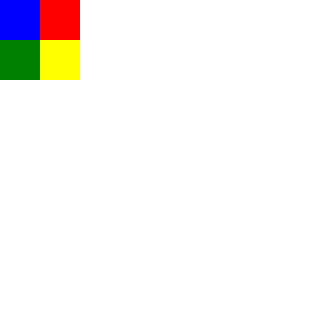
\includegraphics[width=0.15\textwidth]{example}
\end{frame}

\begin{frame}{SVG -- co a jak}
  \begin{itemize}
    \item souřadný systém z levého horního rohu
    \item je potřeba udat celkovou šířku a výšku
    \item zatím nám stačí obdélník -- tag \texttt{rect}
    \item pozor, je to striktní XML, tedy je nutné \texttt{rect} tag uzavřít (!)
    \item vyzkoušejte -- nejdřív jen tak, potom vygenerovat 8x8 mapu (zatím klidně prázdnou)
  \end{itemize}
\end{frame}

\begin{frame}{Další SVG chytrosti}
  \begin{itemize}
    \item kromě \texttt{rect} se bude hodit také \texttt{text}
    \item jako text se zobrazí obsah příslušného elementu
    \item opět použiju atributy \texttt{x}, \texttt{y} (levý dolní roh) a můžu přihodit \texttt{text-anchor=``middle''}, aby to byl dolní prostředek
  \end{itemize}
\end{frame}

\begin{frame}{Postup}
  \begin{itemize}
    \item načtu ze souboru třeba do 2D pole
    \item budu mít hash s barvičkama
    \item vykreslím do SVG
  \end{itemize}
\end{frame}

\begin{frame}{A to je vše, přátelé!}
  \begin{center}
    \includegraphics[width=0.8\textwidth]{looney_tunes}
  \end{center}
\end{frame}

\end{document}
